\documentclass{article}
\usepackage{fontspec}  % Pacchetto per i font in XeLaTeX
\setmainfont{Liberation Serif}  % Imposta il font principale

\usepackage{graphicx}
\usepackage{listings}
\usepackage{xcolor}  % Per il supporto dei colori
\usepackage{tcolorbox}  % Per creare riquadri personalizzati

\usepackage{amsmath, amssymb}
\usepackage{graphicx}
\usepackage{float} % Per usare [H] con figure
\usepackage{caption}
\usepackage{geometry}
\geometry{margin=2.5cm}
\usepackage{booktabs} % Per \toprule, \midrule, \bottomrule nelle tabelle
\usepackage{array} % Per colonne personalizzate in tabular (@{})

% Definizione di un comando per il "backtick style"
\newtcbox{\hi}{on line, nobeforeafter, colframe=gray!60, colback=gray!20, 
    boxrule=0.5pt, arc=3pt, fontupper=\ttfamily, left=2pt, right=2pt, 
    top=2pt, bottom=2pt} 

% Configurazione per il codice
\lstset{
    language=Java,                       % Linguaggio di programmazione
    basicstyle=\ttfamily\small,           % Stile base (monospaziato, dimensione leggermente più grande per chiarezza)
    keywordstyle=\color{teal}\bfseries,   % Parole chiave in verde acqua (modern look) e in grassetto
    stringstyle=\color{orange},       % Stringhe in arancione scuro
    commentstyle=\color{gray}\itshape,    % Commenti in grigio e in corsivo
    numbers=left,                         % Numeri di linea a sinistra
    numberstyle=\tiny\color{gray},        % Numeri di linea piccoli e in grigio
    stepnumber=1,                         % Numerazione di ogni linea
    breaklines=true,                      % Vai a capo automaticamente quando necessario
    tabsize=4,                            % Dimensione del tab
    showstringspaces=false,               % Non mostra spazi negli string literal
    frame=single,                         % Aggiunge una cornice attorno al codice
    backgroundcolor=\color{lightgray!10}, % Sfondo molto leggero e discreto
    morekeywords={String, System, out, println}, % Aggiunta di parole chiave specifiche di Java
    captionpos=b,                         % Posizione della didascalia sotto il codice
    keepspaces=true,                      % Mantiene gli spazi
    emph={public, static, void},          % Parole da enfatizzare
    emphstyle=\color{blue},               % Colore blu per le parole enfatizzate
}



\title{Cheatsheet Statistica}
\author{Giacomo Comitani}
\date{June 2025}

\begin{document}

\maketitle

\section{Modelli Statistici}

\begin{itemize}
    \item \textbf{Bernoulli}: $X \sim B(p)$ : Esperimento avente solamente due possibili esiti: successo o fallimento. \textbf{Discreto}
    \begin{itemize}
        \item Massa: $p^x (1-p)^{1-x} \, \mathbb{I}_{\{0, 1\}}(x)$
        \item Ripartizione: $(1-p) \, \mathbb{I}_{[0,1)}(x) + \mathbb{I}_{[1, +\infty)}(x)$
        \item Valore atteso: $p$
        \item Varianza: $p(1-p)$ 
    \end{itemize}

    \item \textbf{Binomiale}: $X \sim B(n, p)$: Tanti eventi bernoulliani in serie. \textbf{Discreto}
    \begin{itemize}
        \item Massa: $\binom{n}{x} p^x (1-p)^{n-x} \, \mathbb{I}_{\{0, ..., n\}}(x)$
        \item Ripartizione: $\left( \sum_{i=0}^{\lfloor x \rfloor} \binom{n}{i} p^i (1 - p)^{n-i} \right) \mathbb{I}_{[0, n]}(x) + \mathbb{I}_{(n, +\infty)}(x)$
        \item Valore atteso: $n p$
        \item Varianza: $n p(1-p)$
        \item Proprietà: Riproducibilità
        \begin{center}
            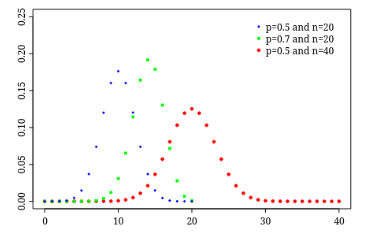
\includegraphics[width=0.4\linewidth]{./immagini/binomiale.png}
        \end{center}
    \end{itemize}

    \item \textbf{Uniforme discreto}: $X \sim U(n)$: Gli esiti della variabile aleatoria sono equiprobabili. \textbf{Discreto}
    \begin{itemize}
        \item Massa: $\frac{1}{n} \, \mathbb{I}_{\{1, ..., n\}}(x)$
        \item Ripartizione: $\frac{\lfloor x \rfloor}{n} \, \mathbb{I}_{[1, n]}(x) + \mathbb{I}_{(n, +\infty)}(x)$
        \item Valore atteso: $\frac{n+1}{2}$
        \item Varianza: $\frac{n^2 - 1}{12}$
        \begin{center}
            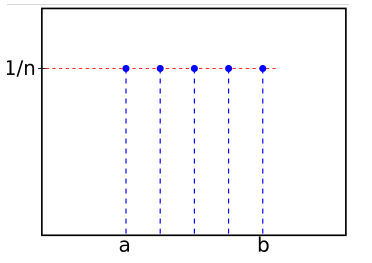
\includegraphics[width=0.4\linewidth]{./immagini/uniformeDiscreto.png}
        \end{center}
    \end{itemize}

    \item \textbf{Geometrico}: $X \sim G(p)$: La variabile assume il numero di insuccessi consecutivi prima che si verifichi un successo in una serie di esperimenti Bernoulliani indipendenti e identicamente distribuiti. \textbf{Discreto}
    \begin{itemize}
        \item Massa: $p(1-p)^x \, \mathbb{I}_{\{0, 1, 2, \dots\}}(x)$
        \item Ripartizione: $\left(1 - (1-p)^{\lfloor x \rfloor + 1} \right) \mathbb{I}_{[0, +\infty)}(x)$
        \item Valore atteso: $\frac{1-p}{p}$
        \item Varianza: $\frac{1-p}{p^2}$
        \item Proprietà: Assenza di memoria
        \begin{center}
            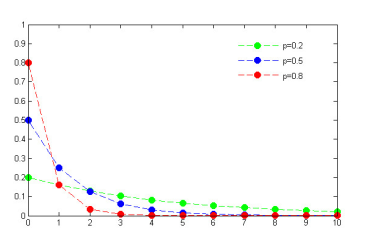
\includegraphics[width=0.4\linewidth]{./immagini/geometrico.png}
        \end{center}
    \end{itemize}

    \item \textbf{Poisson}: $X \sim P(\lambda)$: La variabile assume il numero di eventi che si verificano in un dato intervallo di tempo, sapendo che mediamente se ne verificano un numero $\lambda \in (0, +\infty)$. Tutti gli eventi sono indipendenti. \textbf{Discreto}
    \begin{itemize}
        \item Massa: $\frac{e^{-\lambda} \lambda^x}{x!} \, \mathbb{I}_{\{0, 1, 2, \dots\}}(x)$
        \item Ripartizione: \textit{NON vista nel corso}
        \item Valore atteso: $\lambda$
        \item Varianza: $\lambda$
        \item Proprietà: Approssimazione binomiale, riproducibilità
        \begin{center}
            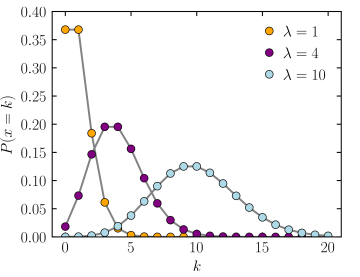
\includegraphics[width=0.4\linewidth]{./immagini/poisson.png}
        \end{center}
    \end{itemize}

    \item \textbf{Ipergeometrico}: $X \sim H(n, M, N)$: La variabile assume il numero di oggetti corretti estratti da un’urna di oggetti binari durante un’estrazione senza reimmissione dopo $n$ estrazioni. \textbf{Discreto}
    \begin{itemize}
        \item Massa: $\frac{\binom{N}{x} \binom{M}{n-x}}{\binom{N+M}{n}} \, \mathbb{I}_{\{0, ..., n\}}(x)$
        \item Ripartizione: \textit{NON vista nel corso}
        \item Valore atteso: $\frac{n N}{N + M}$
        \item Varianza: $\frac{n (N + M - n) N M}{(N+M)^2 (N + M - 1)}$
        \begin{center}
            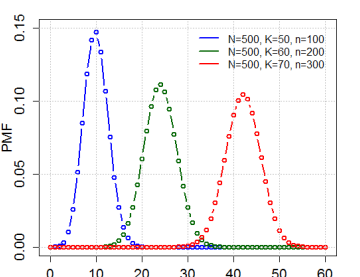
\includegraphics[width=0.4\linewidth]{./immagini/ipergeometrico.png}
        \end{center}
    \end{itemize}

    \item \textbf{Uniforme continuo}: $X \sim U(a,b)$: Gli esiti della variabile aleatoria sono tutti equiprobabili. \textbf{Continuo}
    \begin{itemize}
        \item Densità: $\frac{1}{b-a} \, \mathbb{I}_{[a,b]}(x)$
        \item Ripartizione: $\frac{x-a}{b-a} \, \mathbb{I}_{[a,b]}(x) + \mathbb{I}_{(b, +\infty)}(x)$
        \item Valore atteso: $\frac{a + b}{2}$
        \item Varianza: $\frac{(b-a)^2}{12}$
        \begin{center}
            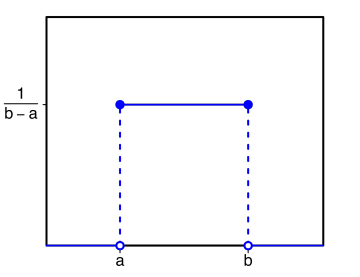
\includegraphics[width=0.4\linewidth]{./immagini/uniformeContinuo.png}
        \end{center}
    \end{itemize}

    \item \textbf{Esponenziale}: $X \sim E(\lambda)$: La variabile assume il tempo di attesa tra due eventi, che mediamente accadono ogni 𝜆 ∈ (0, +∞) unità di tempo. \textbf{Continuo}
    \begin{itemize}
        \item Densità: $\lambda e^{-\lambda x} \, \mathbb{I}_{[0, +\infty)}(x)$
        \item Ripartizione: $\left(1 - e^{-\lambda x} \right) \mathbb{I}_{[0, +\infty)}(x)$
        \item Valore atteso: $\frac{1}{\lambda}$
        \item Varianza: $\frac{1}{\lambda^2}$
        \item Proprietà: Assenza di memoria, scalatura, proprietà su massimo e minimo
        \begin{center}
            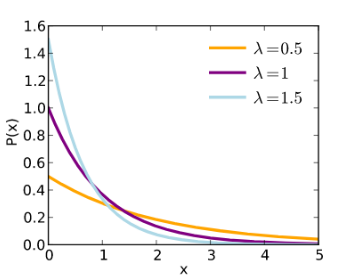
\includegraphics[width=0.4\linewidth]{./immagini/esponenziale.png}
        \end{center}
    \end{itemize}

    \item \textbf{Gaussiana (Normale)}: $X \sim G(\mu, \sigma)$. \textbf{Continuo}
    \begin{itemize}
        \item Densità: $\frac{1}{\sigma \sqrt{2\pi}} e^{-\frac{(x - \mu)^2}{2\sigma^2}}$
        \item Ripartizione: $\int_{-\infty}^{x} \frac{1}{\sigma \sqrt{2\pi}} e^{-\frac{(t - \mu)^2}{2\sigma^2}} \, dt$
        \item Valore atteso: $\mu$
        \item Varianza: $\sigma^2$
        \item Proprietà: Standardizzazione, riproducibilità
        \begin{center}
            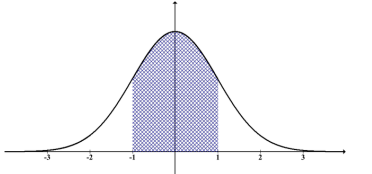
\includegraphics[width=0.4\linewidth]{./immagini/gaussiano.png}
        \end{center}
    \end{itemize}
\end{itemize}

\begin{center}
\begin{tabular}{llp{7.5cm}}
\toprule
\textbf{Distribuzione} & \textbf{Stabile sotto $Y = aX + b$?} & \textbf{Note} \\
\midrule
Bernoulliana           & No    & Il supporto cambia da $\{0,1\}$ a $\{b, a+b\}$; non è più una variabile Bernoulli. \\
Binomiale              & No    & Non resta binomiale: somma di variabili $aX + b$ non ha struttura binomiale. \\
Uniforme discreta      & Sì    & Resta uniforme discreta su un nuovo intervallo: traslazione e scalatura del supporto. \\
Geometrica             & No    & La forma esponenziale viene distrutta dalla trasformazione. \\
Poisson                & No    & Solo somme di variabili Poisson (con stesso $\lambda$) restano Poisson, ma non con $aX + b$. \\
Ipergeometrica         & No    & Modifica la struttura combinatoria; non resta ipergeometrica. \\
Uniforme continua      & Sì    & Resta uniforme continua su un intervallo trasformato: $U(a, b) \rightarrow U(aa + b, ab + b)$. \\
Esponenziale           & Parzialmente & Moltiplicazione positiva ($a > 0$) cambia solo il parametro $\lambda \rightarrow \lambda/a$, ma aggiunta ($b$) rompe la forma. \\
Normale (Gaussiana)    & Sì    & Perfettamente stabile: $X \sim \mathcal{N}(\mu, \sigma^2) \Rightarrow aX + b \sim \mathcal{N}(a\mu + b, a^2\sigma^2)$. \\
\bottomrule
\end{tabular}
\end{center}

\pagebreak

ATTENZIONE ALLA RIPRODUCIBILITÀ: 
\begin{itemize}
    \item BINOMIALE: Le variabili devono essere \textbf{Indipendenti}, il parametro $n$ può essere diverso per ogni variabile, ma il parametro $p$ deve essere uguale!
    \item POISSON: Le variabili devono essere \textbf{Indipendenti}, $X_1 + X_2 \sim P(\lambda_1 + \lambda_2)$. Se le variabili sono anche \textbf{i.i.d.} allora $X_1 + X_2 \sim P(2\lambda)$
    \item NORMALE: Date le variabili aleatorie $X_1, \dots, X_n$ gaussiane e \textbf{indipendenti}, allora: $Y \sim N(\sum_{i = 1}^{n}\mu_i , \sqrt{\sum_{i=1}^{n}\sigma_i^2})$
\end{itemize}

\begin{center}
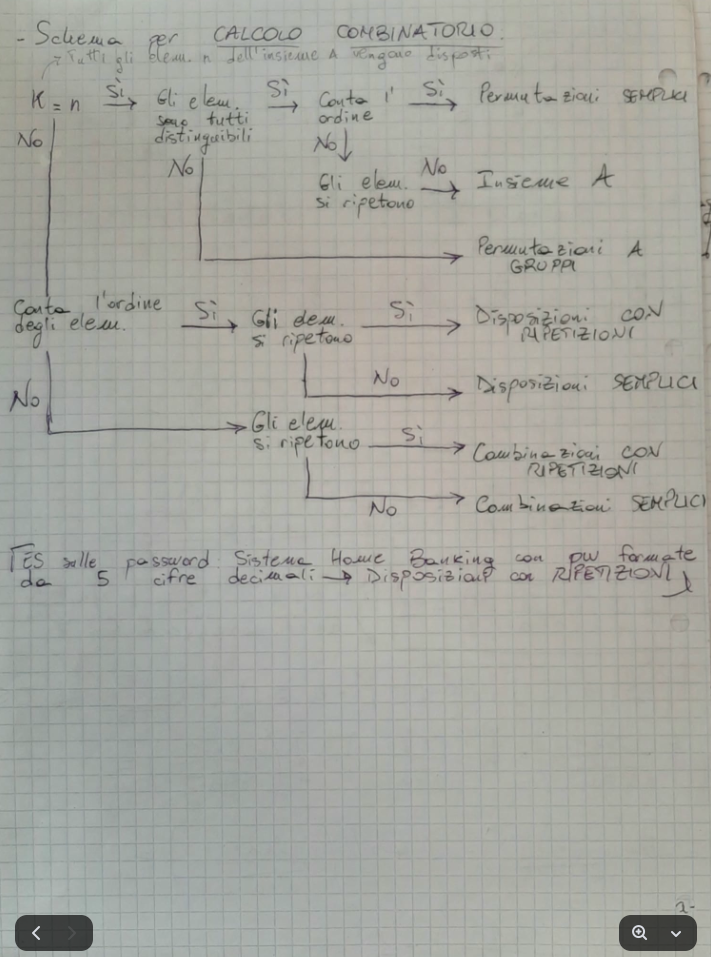
\includegraphics[width=1\linewidth]{./immagini/schemaCombinatorio.png}
\end{center}

\subsubsection{Formule di Calcolo Combinatorio}

\paragraph{Fattoriale}
\[
n! = n \cdot (n-1) \cdot (n-2) \cdots 2 \cdot 1
\]

\paragraph{Permutazioni}

\paragraph{Permutazioni semplici (senza ripetizione)}
\[
P(n) = n!
\]

\paragraph{Permutazioni con ripetizione}
Se alcuni elementi si ripetono:
\[
P(n; n_1, n_2, \ldots, n_k) = \frac{n!}{n_1! \cdot n_2! \cdots n_k!}
\]

\paragraph{Disposizioni}

\paragraph{Disposizioni semplici (senza ripetizione)}
\[
D_{n,k} = \frac{n!}{(n-k)!}
\]

\paragraph{Disposizioni con ripetizione}
\[
D'_{n,k} = n^k
\]

\paragraph{Combinazioni}

\paragraph{Combinazioni semplici (senza ripetizione)}
\[
C_{n,k} = \binom{n}{k} = \frac{n!}{k!(n-k)!}
\]

\paragraph{Combinazioni con ripetizione}
\[
C'_{n,k} = \binom{n+k-1}{k} = \frac{(n+k-1)!}{k!(n-1)!}
\]

\subsubsection{Relazioni utili}
\[
\binom{n}{0} = \binom{n}{n} = 1 \quad \quad \binom{n}{1} = \binom{n}{n-1} = n
\]
\[
\binom{n}{k} = \binom{n-1}{k-1} + \binom{n-1}{k} \quad \text{(relazione di Pascal)}
\]

Espansione del binomio di Newton:
\[
(a + b)^n = \sum_{k=0}^{n} \binom{n}{k} a^{n-k} b^k
\]

\section{Analisi dei dati con python}

\subsection*{Librerie Importanti}

\begin{lstlisting}[language=Python]
    import pandas as pd
    import matplotlib.pyplot as plt
    import numpy as np
    import scipy.stats as st
    import statsmodels.api
    import sklearn
    import itertools
    
\end{lstlisting}
\subsection*{Importazione e caricamento dei dati}

\begin{lstlisting}[language=Python]
import matplotlib.pyplot as plt
import pandas as pd
import numpy as np
import scipy.stats as st

ztl = pd.read_csv('ztl.csv', delimiter=';', decimal='.')
ztl
\end{lstlisting}

\subsection*{Gestione Valori Mancanti}

\begin{lstlisting}[language=Python]
valMancanti = {col: ztl[col].isna().sum() for col in ztl.columns}
dataF = pd.DataFrame(index=valMancanti.keys(), data=valMancanti.values(), columns=['Valori Mancanti'])
dataF
\end{lstlisting}

\subsection*{Visualizzazione dei dati}

La scelta del grafico dipende dalla \textbf{natura del dato} (qualitativo o quantitativo) e dalla \textbf{relazione tra le modalità}.

\subsection*{Dati qualitativi}

\begin{itemize}
  \item \textbf{Grafico a torta (pie chart)}: adatto a variabili \textbf{nominali non ordinabili} (es.\ \texttt{tipo\_motore}). Evidenzia bene le proporzioni tra categorie distinte.
  \begin{lstlisting}[language=Python]
freq = auto['tipo_motore'].value_counts()
freq.plot.pie(autopct='%1.1f%%')
plt.show()
  \end{lstlisting}

  \item \textbf{Grafico a barre (bar plot)}: 
  
  \begin{itemize}
    \item preferibile per variabili \textbf{ordinali} (es.\ \texttt{livello\_rumore}: silenzioso, medio, rumoroso), in cui l'ordine ha significato.
  \begin{lstlisting}[language=Python]
auto['livello_rumore'].value_counts().sort_index().plot.bar()
plt.show()
  \end{lstlisting}
  \item \textbf{Caso binario (es.\ maschio/femmina)}: entrambi i grafici (torta o barre) sono adatti. La torta mostra le proporzioni, le barre facilitano il confronto visivo diretto.
  \end{itemize}
\end{itemize}

\subsection*{Dati quantitativi}

\begin{itemize}
  \item \textbf{Istogramma}: usato per variabili \textbf{continue} (es.\ \texttt{tempo}, \texttt{altezza}), suddivide il dominio in intervalli (bin) e mostra la distribuzione.
  \begin{lstlisting}[language=Python]
data['tempo'].hist(bins=20)
plt.show()
  \end{lstlisting}

  \item \textbf{Grafico a barre o vlines}: usato per variabili \textbf{discrete} (es.\ \texttt{passaggi}), con valori interi distinti. Le \texttt{vlines} sono più leggibili in presenza di molte modalità.
  \begin{lstlisting}[language=Python]
freq = ztl['passaggi'].value_counts()
plt.plot(freq.index, freq, 'o')
plt.vlines(freq.index, 0, freq)
# plt.xlim(0, 30)
plt.show()
  \end{lstlisting}
\end{itemize}


\subsection*{Gestione Outlier}

Per individuare e rimuovere gli outlier posso utilizzare il \hi{boxplot}

\begin{lstlisting}[language=Python]
    # Visualizzarli graficamente
    ztl['passaggi'].plot.box()
    plt.show()

    # Eliminarli dal dataset
    q3 = ztl['passaggi'].quantile(0.75)
    ztl_filtrato = ztl[ztl['passaggi'] <= q3].reset_index(drop=True)
\end{lstlisting}

\subsection*{Tabelle di Frequenza}

\subsubsection*{Congiunta relativa}
\begin{lstlisting}[language=Python]
pd.crosstab(ztl['abbonamento'], ztl['altamente-inquinante'], normalize=True)
\end{lstlisting}

\subsubsection*{Congiunta assoluta}
\begin{lstlisting}[language=Python]
    pd.crosstab(data['attributo 1'], data['attributo 2'])
\end{lstlisting}

\subsubsection*{Relativa semplice}
\begin{lstlisting}[language=Python]
ztl['abbonamento'].value_counts(normalize=True)
\end{lstlisting}

\subsubsection*{Relativa cumulata}

Serve anche a determinare se le due variabili sono \hi{Identicamente distribuite}
\begin{lstlisting}[language=Python]
ztl['passaggi'].value_counts(normalize=True).sort_index().cumsum()
\end{lstlisting}

\subsubsection*{Cumulata con binning}
\begin{lstlisting}[language=Python]
auto['numero_occupanti'].value_counts(normalize=True, bins=10).sort_index().cumsum()
\end{lstlisting}

\subsection*{Correlazione}

\begin{lstlisting}[language=Python]
plt.scatter(accessi['allarme2'], accessi['carico_sistema'])
plt.show()
\end{lstlisting}


\begin{itemize}
    \item ris $\to$ +1 probabile correlazione linearmente diretta
    \item ris $\to$ 0 correlazione improbabile
    \item ris $\to$ −1 probabile correlazione linearmente indiretta
\end{itemize}

\subsection*{Filtraggio Dati}

\begin{lstlisting}[language=Python]
    ztl_giornalieri = ztl[ztl['abbonamento'] == 0]
\end{lstlisting}

\subsection*{Indici Statistici}

\subsubsection*{Gini per concentrazione}
\begin{lstlisting}[language=Python]
    def gini_concentrazione(series):
        freqs = series.value_counts(normalize=True).sort_values().values
        n = len(freqs)
        if n < 2: return 0.0
        Q = np.cumsum(freqs)[:-1]
        F = np.arange(1, n) / n
        return (F - Q).sum() / F.sum()

    gini_concentrazione(auto['tipo_motore'].dropna())
\end{lstlisting}

\subsubsection*{Gini per eterogeneità}
\begin{lstlisting}[language=Python]
def gini2(series):
    return 1 - sum(series.value_counts(normalize=True).map(lambda f: f ** 2))

gini2(auto['tipo_motore'])
\end{lstlisting}

\subsection*{Conversione booleana per correlazioni}

\begin{lstlisting}[language=Python]
data['convertito'] = data['da_convertire'].apply(lambda x: x == 'ON')
\end{lstlisting}

\subsection*{Indici Statistici}

\subsubsection*{Indici di centralità}

\paragraph{}{Moda di un carattere}


\begin{lstlisting}
data['attributo'].mode()
\end{lstlisting}

\paragraph{}{Media campionaria di un carattere}

\begin{lstlisting}
data['attributo'].mean()
\end{lstlisting}

\paragraph{}{Mediana di un carattere}

\begin{lstlisting}
data['attributo'].median()
\end{lstlisting}

\subsubsection*{Indici di dispersione}

\paragraph{}{Varianza campionaria}

\begin{lstlisting}
data['attributo'].var()
\end{lstlisting}

\paragraph{}{deviazione standard campionaria}

\begin{lstlisting}
data['attributo'].std()
\end{lstlisting}

\subsection*{Analisi Dataset}

\subsubsection*{Elemento massimo}

\begin{lstlisting}
dato = data[data['attributo'] == max(data['attributo'])]
\end{lstlisting}

\subsubsection*{Elemento minimo}

\begin{lstlisting}
dato = data[data['attributo'] == min(data['attributo'])]
\end{lstlisting}

\subsubsection*{Valori assumibili da un carattere}

\begin{lstlisting}
list(data['attributo'].unique())
\end{lstlisting}

\subsubsection*{Tipo e forza di correlazione}

\begin{lstlisting}
data['attributo'].std()
\end{lstlisting}

\subsubsection*{QQ Plot attributo-normale}

\begin{lstlisting}
    import statsmodels.api as sm
    mu = data['attributo_1'].mean()
    sigma = data['attributo_1'].std()
    sm.qqplot(data['attributo_1'],dist = st.norm, line = '45', loc = mu, scale = sigma)
    plt.show()  
\end{lstlisting}

\subsubsection*{QQ Plot tra due attributi }

\begin{lstlisting}
    import statsmodels.api as sm 

    sm.qqplot_2samples(data['attributo_1'], data['attributo_2'], line = '45')
    plt.show()
\end{lstlisting}

\subsubsection*{QQ Plot attributo-distribuzione qualsiasi discreta}

\begin{lstlisting}
    import statsmodels .api as sm

    mu = allarme_si_finale.mean()

    sm.qqplot(allarme_si_finale, dist=st.poisson(mu), line='45')
    plt.show()
\end{lstlisting}



\subsubsection*{PiePlot}

\begin{lstlisting}
    freq = data['c1'].value_counts()
    df = pd.DataFrame({'freq':freq})
    print(df)

    freq.plot.pie()
    plt.show()
\end{lstlisting}

\subsubsection*{Grafico a barre}
\begin{lstlisting}
    freq_punteggio = data['attributo'].value_counts()
    plt.bar(freq_punteggio.index, freq_punteggio.values)
    plt.show()
\end{lstlisting}

\subsubsection*{Individuazione outlier (visivamente)}

In questo caso conviene fare il box plot che posso fare con:

\begin{lstlisting}
    ztl['passaggi'].plot.box()
    plt.show()
\end{lstlisting}

\subsubsection*{Rimozione degli outlier}

\begin{lstlisting}
    # guardo boxplot
    data = data[data['attributo'] <= data['attributo'].quantile(0.75)].reset_index(drop = True)
\end{lstlisting}

\subsubsection*{Correlazione tra due attributi}

- Faccio \hi{.corr} per usare \hi{Pearson} e poi confermo ipotesi con uno scatter:

\begin{lstlisting}
    ztl.plot.scatter('abbonamento', 'passaggi')
    plt.show()
\end{lstlisting}

A seconda del risultato $ris$ ottenuto:

\begin{itemize}
    \item ris $\to$ +1 probabile correlazione linearmente diretta
    \item ris $\to$ 0 correlazione improbabile
    \item ris $\to$ -1 probabile correlazione linearmente indiretta
\end{itemize}

\subsubsection*{ScatterPlot (2 parametri)}

\begin{lstlisting}
    data.plot.scatter('attrinbuto_1', 'attributo_2')
\end{lstlisting}

\subsubsection*{ScatterPlot (3 parametri)}

\begin{lstlisting}
    heroes[heroes['Gender']=='M'].plot.scatter('Height', 'Weight')
    plt.show()
\end{lstlisting}

\subsubsection*{Tabella delle frequenze relative cumulate}

\begin{lstlisting}[language=Python]
    freq_rel_cumulate = auto['numero_occupanti'].value_counts(normalize = True).sort_index().cumsum()

    # Qui il prof preferisce utilizzare i bins, occhio pero che cosi restituisce un 
    # intervallo e non un valore, quindi per i calcoli meglio usare senza bins

    freq_rel_cumulate_print_prof = auto['numero_occupanti'].value_counts(normalize = True, bins = 10).sort_index().cumsum()

    freq_rel_cumulate_print_prof
\end{lstlisting}

\subsubsection*{Tabella delle frequenze relative NON cumulate}

\begin{lstlisting}
    freq_rel_carpooling = auto_ridotto['carpooling'].value_counts(normalize = True)
    freq_rel_carpooling
\end{lstlisting}

\subsubsection*{Convertire valore da stringa a booleano}

\begin{lstlisting}
    accessi['allarme2'] = accessi['allarme'].apply(lambda x : x == 'ON')

    accessi['carico_sistema'].corr(accessi['allarme2'])
\end{lstlisting}

\subsubsection*{Calcolo dimensione del campione togliendo tutti gli elementi mancanti}

\begin{lstlisting}
    campione_senza_null = ztl_giornalieri['passaggi'] - ztl_giornalieri['passaggi'].isnull().sum()
    n = len(campione_senza_null)
\end{lstlisting}

\subsubsection*{Linespace e Arange}

\begin{itemize}
    \item \textbf{linespace}: np.linespace(start, stop, num), dove num è il numero di punti da generare nell'intervallo specificato
    \item \textbf{arange}: np.arange(start, stop, step), dove step è l'incremento tra i valori consecutivi (se omesso è uguale a 1)
\end{itemize}

\subsubsection*{Aggiunta nuovo attributo nel dataset}

\begin{lstlisting}[language=Python]
    # il nuovo attributo dev'essere chiamato punteggio ed è dato dal doppio delle basse emissioni - carpooling:
    lista_nuovo_attributo = (2 * auto['basse_emissioni'] - auto['carpooling'].to_numpy())

    auto['punteggio'] = lista_nuovo_attributo

    # stampa del nuovo attributo aggiunto al dataset:
    auto['punteggio']
\end{lstlisting}

\subsubsection*{individuazione e rimozione valori nulli}

\begin{lstlisting}[language=python]
    # Prima di tutto verifico che non ci siano valori nulli:
    print(ztl_giornalieri['categoria'].isnull().sum())

    # Eventualmente per toglierli
    senza_nulli = ztl_giornalieri.dropna(subset=['categoria'])

    print(senza_nulli['categoria'].isnull().sum())
\end{lstlisting}



\pagebreak

\section{calcolo probabilità}

Ricordiamo innanzitutto che, se ad esempio ci viene chiesto di calcolare $P(X > 30)$:

\[
P(X > 30) = 1 - P(X \leq 30)
\]

Il problema si pone quando la richiesta è di calcolare $P(X \geq 30)$:

\begin{itemize}
  \item Nel caso delle \textbf{variabili aleatorie discrete}, il calcolo diventa:
  \[
  P(X \geq 30) = 1 - P(X \leq 29)
  \]
  poiché $P(X \geq 30) = P(X = 30) + P(X = 31) + \dots$.

  \item Nel caso delle \textbf{variabili aleatorie continue}, non si pone questo problema, perché:
  \[
  P(X = 30) = 0
  \]
  quindi si può scrivere semplicemente:
  \[
  P(X \geq 30) = P(X > 30) = 1 - P(X \leq 30)
  \]
\end{itemize}

\subsection*{}{Proprietà del valore atteso}

Posto ad esempio $Z = 2X - Y$:

\begin{itemize}
    \item \textbf{Valore atteso} = $E[Z] = E[2X - Y] = E[2X] - E[Y] = 2 \cdot p - p = 2p - p = p$
    \item \textbf{Varianza}:  $Var(Z) = Var(2X - Y) = Var(2X) + Var(-Y) = 4 \cdot Var(X) + Var(Y) = 4 \cdot [p(1-p)] + [p(1-p)] = 4 \cdot (p - p^2) + [p - p^2] = 4p - 4p^2 + p - p^2 = -5p^2 + 5p = 5p(1 - p)$
\end{itemize}

\subsection*{Proprietà della varianza}

La varianza della funzione indicatrice è la probabilità dell'evento moltiplicata per la probabilità dell'evento complementare:

$VAR(I) = P(A) * P(\overline{A})$

La varianza NON opera in modo lineare: $VAR(aX + b) = a^2 VAR(X)$

La varianza della somma di due variabili aleatorie $X$ e $Y$ vale:

\begin{itemize}
    \item $VAR(X + Y) = VAR(X) + VAR(Y) + 2COV(X,Y)$
    \item $VAR(X - Y) = VAR(X) + VAR(Y) - 2COV(X,Y)$
\end{itemize}

Se le due variabili sono \textbf{indipendenti identicamente distribuite}, allora la covarianza vale zero, quindi le formule di prima diventano:

\begin{itemize}
    \item $VAR(X + Y) = VAR(X) + VAR(Y)$
    \item $VAR(X - Y) = VAR(X) + VAR(Y)$
\end{itemize}

Ricordo che la varianza della media campionaria vale: $VAR(\overline{X}) = \frac{VAR(X)}{n}$

Ricordo infine che $COV(X, Y) = E[XY] - E[X]E[Y]$

\pagebreak

\section{Esercizio 1}

\subsubsection*{Visualizzare Graficamente una variabile aleatoria/ Visualizzarne le specificazioni}

\begin{lstlisting}
    import numpy as np
    import matplotlib.pyplot as plt
    import pandas as pd
    import scipy.stats as st

    # Modifica i parametri
    p = 0.7
    n = 30
    num_sample = 100000

    # Modifica la distribuzione
    binom = st.binom(n, p)
    X = binom.rvs(num_sample)

    # Modifica La variabile aleatoria
    Z = 2 * X

    specificazioni, freq_assolute = np.unique(Z, return_counts = True)
    print("Specificazioni: ", specificazioni)
    print("Numero di occorrenze per specificazione: ", freq_assolute)

    pmf = freq_assolute / num_sample
    plt.stem(specificazioni, pmf)

    plt.show()
\end{lstlisting}


\subsubsection*{Tracciare una funzione generica}

\begin{lstlisting}
    import pandas as pd
    import scipy.stats as st
    import numpy as np
    import matplotlib.pyplot as plt

    h = 4/10

    def f(x):
        return (1-(1-h)**(x+1))

    x = np.linspace(1, 30, 100)
    y = [f(n) for n in x]


    plt.plot(x, y)

    plt.grid(True)
    plt.show()
\end{lstlisting}

\pagebreak

\subsubsection*{Dimostrare che f è una funzione di densità}


Sappiamo che la funzione di densità deve rispettare le seguenti proprietà:

\begin{itemize}
    \item $f_X(x) \geq 0$
    \item $\int_{-\infty}^{\infty}f_X(x) dx = 1$

\end{itemize}

\subsection*{La descrizione data di $f$ permette di dire che la distribuzione di $X$ è approssimabile in modo accettabile usando il teorema centrale del limite? Giustificare il ragionamento}

Sappiamo che la variabile aleatoria X ha media finita, (abbiamo calcolato sopra il valore atteso), e quindi ha varianza finita. Inoltre so che il supporto è finito, quindi posso applicare il teorema centrale edel limite per approssimare X in modo accettabile.

\subsection*{Verificare che $f$ sia una funzione di massa}

La funzione di massa è una funzione $f$ che deve rispettare le seguenti proprietà:

\begin{itemize}
    \item Non può essere negativaù
    \item La somma dei valori della funzione di massa per tutti gli x deve fare 1
\end{itemize}
\subsection*{Indicate i valori di $a$ e $b$ per i quali $Z$ risulta essere una variabile aleatoria, motivando la vostra risposta}

Una variabile aleatoria è una quantità il cui valore non può essere predeterminato con certezza ma è soggetto a variazioni casuali, ovvero che ha un valore NON costante.

Nel nostro caso, Z è una variabile aleatoria per ogni $a, b \in R$. Tuttavia, nel caso in cui `a = 0` e `b = 0`, la variabile `Z` assume sempre valore `Z = 0` con probabilità = 1, quindi diventa una variabile aleatoria degenere

\subsection*{Formule della varianza}

\begin{itemize}
    \item $VAR(aX) = a^2* VAR(X)$
    \item $VAR(X + b) = VAR(X)$
    \item $VAR(\overline {X}) = \frac{VAR(X)}{n}$
    \item $VAR(X) = E[X^2] - E[X]^2$
\end{itemize}

\section{Esercizio 2}

\begin{itemize}
    \item Stimatore non deviato: valore atteso è uguale al parametro che voglio stimare
    \item Stimatore deviato: valore aatteso NON è uguale al parametro che voglio stimare
    \item Determinare stimatore non distorto:
    \begin{itemize}
        \item Se riesco uso plug-in 
        \item Se nell'appliczione del plug-in ho operatori non lineari, uso metodo di massima verosimiglianza
    \end{itemize}
\end{itemize}

Se nell'appliczione del plug-in ho operatori non lineari, uso metodo di massima verosimiglianza

\subsection*{MSE}

Scarto quadratico medio (MSE) = $VAR(Stimatore) + Bias^2(Stimatore)$

Consistenza in media quadratica:

\begin{itemize}
    \item $\lim_{n \to \infty}MSE = 0$: gode della proprietà
    \item $\lim_{n \to \infty}MSE \neq 0$: NON gode della proprietà
\end{itemize}

\subsection*{Il metodo di Massima Verosimiglianza}

Oltre al metodo plug-in, potrei utilizzare il metodo di massima verosimiglianza nel caso in cui avessi operatori non lineari. \\

Per capire come utilizzarlo correttamente, partiamo da questi assunti:

\begin{itemize}
    \item $f_X (x) \to$ Funzione di Massa/Densità di Probabilità \textbf{Marginale}.
    \item $f_X(x_i) = L(p) = \prod_{i=1}^{n} f_X(x_i, p) \to$ Funzione di Massa/Densità di Probabilità \textbf{Congiunta}.
\end{itemize}

Esempio con Funzione di Massa di Probabilità Marginale della distribuzione Bernoulliana, a partire dalla quale voglio stimare un parametro fissato $p$: \\

La Funzione Marginale è: $f_X(x) = p^x (1-p)^{1-x}$, con $X \in \{0,1\}$ \\

La Funzione Congiunta è invece: $L(p) = \prod_{i=1}^{n} f_X(x_i, p) = p^{\sum_{i=1}^{n}x_i} (1-p)^{n-\sum_{i=1}^{n} x_i}$ \\

A questo punto bisogna utilizzare le proprietà del \textbf{logaritmo naturale} per non avere le sommatorie come esponenti:\\


$\Rightarrow \ln[L(p)] = ln[p^{\sum_{i=1}^{n}x_i} (1-p)^{n-\sum_{i=1}^{n} x_i}] \Rightarrow$ \\
\\
$\Rightarrow \ln[p^{\sum_{i=1}^{n}x_i} (1-p)^{n-\sum_{i=1}^{n} x_i}] = \sum_{i=1}^{n} x_i \cdot \ln(p) + (n - \sum_{i=1}^{n} x_i) \ln(1-p) =$ \\

Ora devo:
\begin{itemize}
    \item Derivare rispetto al parametro che intendiamo stimare (in questo caso è $p$);
    \item Uguagliare il tutto a 0 ed isolare il parametro da stimare.
\end{itemize}

$\Rightarrow \sum_{i=1}^{n} x_i \cdot \frac{1}{p} - (n - \sum_{i=1}^{n} x_i) \frac{1}{1-p} = 0 \Rightarrow$ \\
\\
$\Rightarrow \sum_{i=1}^{n} \frac{x_i}{p} = \frac{n-\sum_{i=1}^{n} x_i} \Rightarrow$ \\
\\
$\Rightarrow \frac{\sum_{i=1}^{n} x_i (1-p)}{p(1-p)} = \frac{np - (\sum_{i=1}^{n} x_i)p}{p(1-p)}$ \\
\\
$\Rightarrow p = \frac{1}{n} \sum_{i=1}^{n} x_i \to$ che è la \textbf{media campionaria} di $X$, per definizione stimatore \textbf{non distorto} per $p$.

\subsection*{Applicare il teorema centrale del limite}

$P(|T - p| \leq \epsilon)$ = $2\Phi(\frac{\epsilon\sqrt{n}}{\sigma}) - 1$

Se mi chiede la taglia minima del campione: risolvo per $n$

\subsection*{Utilizzando il teorema centrale del limite, determinate la distribuzione approssimata dello stimatore $T$ che avete ottenuto al punto 5}

Il teorema centrale del limite afferma che, per $n$ grande:

$\overline{X} \sim N(\mu, \frac{\sigma^2}{n})$

Sappiamo però che T = 2* $\overline{X}$, quindi, per le propietà delle trasformazioni lineari delle normali, possiamo dire che:

$T \sim N (2 \mu, \frac{4 \sigma^2}{n})$

\subsection*{I dati a disposizione permettono di garantire, con probabilità maggiore o uguale a 0.99, che la stima fatta nell'Esercizio 5.2 comporti un errore (in valore assoluto) di massimo $\epsilon = 0.1$}

A questo punto devo:

\begin{itemize}
    \item Calcolare la taglia minima del camoione isolando la n
    \item Calcolare la taglia del campione effettivo (occhio ad eliminare eventuali valori nulli)
    \item Confrontare i valori: se il \textbf{Secondo valore} è >= del primo, allora la stima è \textbf{affidabile}
\end{itemize}


\subsection*{Formule Utili}

$E[X^2] = \sum_{i}(x_i)^2*p(x_i)$

\pagebreak

\section{Esercizio 3}

\subsubsection*{Grafico empirico della funzione di ripartizione}

\begin{lstlisting}[language=Python]
    # Estrai e ordina i valori della colonna 'richieste'
    richieste = accessi['richieste'].sort_values().values
    n_total = len(richieste)

    # Calcola la CDF empirica (y = frazione cumulativa)
    y = np.arange(1, n_total + 1) / n_total  # Frazione cumulativa (es. 0.2, 0.4, ..., 1.0)

    # Crea il grafico ECDF
    plt.step(richieste, y, label = 'ECDF')
    plt.xlabel('Numero di Richieste')
    plt.ylabel('Frazione Cumulativa (CDF)')
    plt.title('Distribuzione Cumulativa delle Richieste')
    plt.grid(True, linestyle='--', alpha=0.7)

    # Esempio: traccia una linea orizzontale per un f specifico (es. f=95%)
    f = 95
    plt.axhline(y = f/100, color='red', linestyle='--', label=f'{f}% dei casi')
    plt.legend()

    plt.show()
\end{lstlisting}

\subsubsection*{Fissato un generico numero $f$ compreso fra 0 e 100, vogliamo determinare il numero $n$ che rende vera l'affermazione nell'$f$ percento dei casi sono arrivate al massimo $n$ richieste"}

\begin{lstlisting}
    f = 95
    richieste = accessi['richieste'].sort_index()
    richieste.quantile(f/100)
\end{lstlisting}
\section{Calcolo combinatorio python}

\subsubsection*{utilità}

\begin{lstlisting}
    from math import factorial as fact
    from scipy.special import binom
    # fattoriale
    fact(5) # 120
    # coefficiente binomiale
    binom(5, 2) # 10
\end{lstlisting}

\subsubsection*{combinazioni/disposizioni/permutazioni}

\begin{lstlisting}
    # N = numerosità insieme da cui pescare
    # k = numero oggetti da estrarre
    from scipy.special import comb, perm
    # combinazioni, con o senza ripetizioni (ordine non conta)
    comb(N, k, repetition=False)
    # disposizioni (o permutazioni in caso k = N) SENZA RIPETIZIONI (ordine conta)
    perm(N, k)
\end{lstlisting}

\pagebreak

\section*{Appendice statistica}

\subsection*{Correzione Bessel}
Usa la correzione di Bessel quando:
\begin{itemize}
    \item Hai un \textbf{campione} di dati
    \item Vuoi stimare la \textbf{deviazione standard della popolazione} ($\sigma$)
\end{itemize}

\subsection*{Formule}
\begin{tabular}{|l|l|}
\hline
\textbf{Popolazione} (σ nota) & $\sigma = \sqrt{\dfrac{1}{N}\sum\limits_{i=1}^N (x_i - \mu)^2}$ \\
\hline
\textbf{Campione} (stima di σ) & $s = \sqrt{\dfrac{1}{n-1}\sum\limits_{i=1}^n (x_i - \bar{x})^2}$ \\
\hline
\end{tabular}

\subsection*{Perché $n-1$?}
\begin{itemize}
    \item Corregge il \textbf{bias} nella stima
    \item $n-1$ = gradi di libertà (perdiamo 1 grado usando $\bar{x}$)
    \item Senza correzione si \textbf{sottostima} σ
\end{itemize}

\subsection*{Implementazione}
\begin{lstlisting}
import numpy as np
s = np.std(dati, ddof=1)  # ddof=1 -> divide per (n-1)
\end{lstlisting}

\subsection*{Proprietà della Media Campionaria}

Data un campione $X_1, X_2, \dots, X_n$, dove le variabili sono \hi{i.i.d.} la media campionaria è:
\[
\bar{X} = \frac{1}{n} \sum_{i=1}^{n} X_i
\]

\begin{itemize}
  \item \textbf{Stima imparziale:} 
  \[
  \mathbb{E}[\bar{X}] = \mu
  \]
  La media campionaria è una stima imparziale della media della popolazione.

  \item \textbf{Varianza:}
  \[
  \mathrm{Var}(\bar{X}) = \frac{\sigma^2}{n}
  \]
  La varianza diminuisce all'aumentare della dimensione del campione.

  \item \textbf{Distribuzione asintotica (Teorema del Limite Centrale):}
  \[
  \bar{X} \xrightarrow{d} \mathcal{N} \left( \mu, \frac{\sigma^2}{n} \right) \quad \text{per } n \to \infty
  \]

  \item \textbf{Efficienza:} 
  Tra le stime imparziali della media, $\bar{X}$ ha varianza minima sotto certe condizioni.
\end{itemize}

\subsection*{Funzione di Ripartizione (CDF)}

Data una variabile casuale $X$, la funzione di ripartizione è definita in generale come:
\[
F_X(x) = \mathbb{P}(X \leq x)
\]

\subsubsection*{Caso Discreto}
Se $X$ è discreta e assume valori $x_1, x_2, \dots$, con funzione di massa di probabilità $p_X(x_i) = \mathbb{P}(X = x_i)$, allora:
\[
F_X(x) = \sum_{x_i \leq x} p_X(x_i)
\]

\begin{itemize}
  \item $F_X(x)$ è una funzione a gradini
  \item È destra-continua
  \item Cresce solo nei punti $x_i$ dove $X$ ha massa di probabilità
\end{itemize}

\subsubsection*{Caso Continuo}
Se $X$ è continua con densità di probabilità $f_X(x)$, allora:
\[
F_X(x) = \int_{-\infty}^{x} f_X(t) \, dt
\]

\begin{itemize}
  \item $F_X(x)$ è continua
  \item Se derivabile, vale: $f_X(x) = \frac{d}{dx}F_X(x)$
  \item La probabilità in un punto è nulla: $\mathbb{P}(X = x) = 0$
\end{itemize}

\subsubsection*{Proprietà Comuni}
\begin{itemize}
  \item $\lim\limits_{x \to -\infty} F_X(x) = 0$
  \item $\lim\limits_{x \to +\infty} F_X(x) = 1$
  \item $F_X(x)$ è monotona non decrescente
  \item È destra-continua
\end{itemize}

\subsection*{${E}[X^2]$}

\subsection*{Caso Discreto}
Se $X$ è discreta con funzione di massa $p_X(x)$:
\[
\mathbb{E}[X^2] = \sum_{x \in \text{Im}(X)} x^2 \cdot p_X(x)
\]

\subsection*{Caso Continuo}
Se $X$ è continua con densità di probabilità $f_X(x)$:
\[
\mathbb{E}[X^2] = \int_{-\infty}^{+\infty} x^2 \cdot f_X(x) \, dx
\]

\end{document}